% !TEX root = ../master_thesis.tex
\chapter{Compléments au chapitre~\ref{chap:théorie}}\label{annexe:théorie}

\section{Codes et ressources de calcul}\label{sec:annexe_codes}

Les paramètres numériques des calculs du mémoire sont rapportés à la fin des annexes de chaque chapitre. Dans chaque tableau, la colonne \og Section \fg{} renvoie à l'endroit du texte où la valeur est donnée. Une valeur qui diffère d'une chaîne à l'autre est donnée dans chaque tableau. Les calculs DFT et DFPT sont réalisés avec \texttt{QuantumESPRESSO} (version~7.4.1), le calcul des fonctions de Wannier avec \texttt{Wannier90} (version~3.1.0) et \texttt{EPW} (version~6.0), et le post-traitement des données est effectué en Python (version~3.11.5) avec \texttt{NumPy} (version~1.26.4) et \texttt{SciPy} (version~1.15.2).

Tous les calculs ont été effectués sur la grappe Rorqual de l'Alliance de recherche numérique du Canada et Calcul Québec. Le dépôt GitHub \href{https://github.com/Gregb26/msc-graphene-raman-defects}{\texttt{msc-graphene-raman-defects}} contient les fichiers d'entrée de chaque calcul dans le dossier \texttt{calculs/}, puis les scripts dans \texttt{scripts/} et les données dans \texttt{donnees/} servant à la génération des figures du mémoire. Le code de recherche ayant servi à générer les données se trouve dans un dépôt GitHub privé et est disponible sous demande.

\clearpage
\section{Expressions explicites de la fonctionnelle PBE}\label{annexe:pbe}

Dans cette annexe, nous donnons les expressions explicites propres à la fonctionnelle d'échange-corrélation PBE~\cite{perdewGeneralizedGradientApproximation1996a} que nous utilisons dans tous les calculs de ce mémoire. Toutes les expressions données ici sont écrites dans les unités atomiques d'Hartree, où
\begin{equation}
    \hbar = e = 4\pi\varepsilon_0 = m_e = 1.
    \label{eqn:a1_unités_hartree}
\end{equation}
La PBE est une fonctionnelle GGA qui prend la forme suivante
\begin{equation}
    E_\text{XC}^\text{PBE}[n]=\int d^3\rv\,n(\rv)\left[\varepsilon_\text{X}^\text{hom}(n)F_\text{X}(n,\nabla n)+\varepsilon_\text{C}^\text{hom}(n)F_\text{C}(n,\nabla n)\right],
    \label{eqn:a1_EPBE}
\end{equation}
où $\varepsilon_\text{X/C}^\text{hom}(n)$ est la densité d'énergie d'échange/corrélation d'un gaz d'électrons homogène de densité $n$ et $F_\text{X/C}(n,\nabla n)$ est un facteur d'amplification adimensionnel pour l'échange/corrélation qui dépend du gradient de la densité et qui se réduit à l'unité dans la limite de la LDA.

La partie d'échange d'un gaz d'électrons homogène est connue analytiquement et est donnée par~\cite{martinElectronicStructureBasic2004}
\begin{equation}
    \varepsilon_\text{X}^\text{hom}(n)=-\frac{3}{4\pi}\left(\frac{9\pi}{4}\right)^{1/3}\frac{1}{r_s},
    \label{eqn:a1_eX}
\end{equation}
pour un système qui n'est pas polarisé en spin. Ici, $r_s$ est le rayon de Wigner-Seitz qui est défini comme le rayon de la sphère contenant en moyenne un électron pour un gaz de densité $n$
\begin{equation}
    r_s = \left(\frac{3}{4\pi n}\right)^{1/3}.
    \label{eqn:a1_rs}
\end{equation}
C'est un paramètre naturel pour caractériser la densité d'un gaz homogène. Le facteur d'amplification $F_\text{X}$ pour l'échange est donné par
\begin{equation}
    F_\text{X}(n,\nabla n)=1+\kappa-\frac{\kappa}{1+\mu s^2/\kappa},
    \label{eqn:a1_FX}
\end{equation}
où le paramètre $s$ est proportionnel au gradient de la densité
\begin{equation}
    s=\frac{|\nabla n|}{2k_Fn}.
\end{equation}
Ici, $\kappa$ et $\mu$ sont des paramètres à déterminer à partir des contraintes théoriques sur la fonctionnelle d'échange-corrélation et $k_F=(3\pi^2n)^{1/3}$ est le vecteur d'onde de Fermi pour un gaz d'électrons uniforme. Lorsque nous négligeons le gradient de la densité, c'est-à-dire quand $s=0$, nous avons que $F_\text{X}=1$ et nous retrouvons bien la LDA pour l'échange.

La partie de corrélation de la densité d'énergie d'un gaz d'électrons homogène n'est pas connue analytiquement. Elle a plutôt été calculée numériquement, avec haute précision, par Ceperley et Alder~\cite{ceperleyGroundStateElectron1980} à l'aide de la méthode stochastique Monte-Carlo quantique puis paramétrée par Perdew et Zunger~\cite{perdewSelfinteractionCorrectionDensityfunctional1981}. Nous référons le lecteur à ce dernier article pour cette paramétrisation. Le facteur d'amplification pour la corrélation $F_\text{C}$ est donné par
\begin{equation}
    \label{eqn:a1_FC}
    F_\text{C}(n,\nabla n) = 1+H(t)/\varepsilon_\text{C}^\text{hom}(n).
\end{equation}
La fonction $H(t)$ est définie comme étant
\begin{equation}
    H(t) = \gamma\phi^3\log\left(1+\frac{\beta}{\gamma}t^2\left[\frac{1+At^2}{1+At^2+A^2t^4}\right]\right),
    \label{eqn:a1_Ht}
\end{equation}
où $t$ est un autre paramètre proportionnel au gradient de la densité
\begin{equation}
    t = \frac{|\nabla n|}{2\phi k_Sn}.
\end{equation}
Ici, $\gamma$ et $\beta$ sont d'autres paramètres à déterminer à l'aide des contraintes, $k_S=(4k_F/\pi)^{1/2}$ est le vecteur d'onde d'écrantage de Thomas-Fermi, et les quantités $\phi$ et $A$ sont données par
\begin{align}
    \phi &= \frac{(1+\zeta)^{2/3}+(1-\zeta)^{2/3}}{2},\\
    A &= \frac{\beta}{\gamma}\left[\exp\left(-\frac{\varepsilon_\text{C}^\text{hom}}{\gamma\phi^3}\right)-1\right]^{-1},
\end{align}
où $\zeta=(n_\uparrow-n_\downarrow)/n$ est la polarisation en spin. Pour les systèmes non polarisés en spin comme le graphène que nous étudions dans ce mémoire : $n_\uparrow = n_\downarrow$ et donc $\zeta=0$, ce qui veut dire que $\phi=1$. Encore une fois, si nous ignorons le gradient de la densité, c'est-à-dire quand $t=0$, nous avons que $H(t=0)=0$ et que $F_\text{C}=1$ et nous retombons sur la LDA. Il est important de comprendre que la fonctionnelle XC PBE ne dépend pas de données empiriques, malgré ce que les paramètres à déterminer $\kappa, \mu,\gamma$ et $\beta$ peuvent laisser présager. En effet, ces paramètres sont déterminés à partir de conditions théoriques que doivent satisfaire les termes d'échange et de corrélation. Ces conditions sont explicitées dans l'article original de la PBE~\cite{perdewGeneralizedGradientApproximation1996a} et pour satisfaire ces contraintes, les paramètres doivent prendre les valeurs approximatives $\kappa=0.804$, $\mu=0.21951$, $\gamma=0.031091$ et $\beta=0.066725$. La fonctionnelle XC PBE est ainsi entièrement déterminée par la théorie, sans ajustement empirique.

\clearpage
\section{Convergence de l'état fondamental électronique}\label{sec:annexe_conv_dft}

La figure~\ref{fig:convergence_dft} rassemble les tests de convergence de l'état fondamental électronique du graphène parfait (section~\ref{sec:electron_results}) : coupure $E_\text{cut}$, grille $\kv$ et schéma d'occupation, avec le seuil de $0.1$~meV par atome.

L'énergie est variationnelle par rapport à $E_\text{cut}$ et décroît de façon monotone. La première coupure sous le seuil est $E_\text{cut}=100$~Ry (panneau (a)). Toutefois, elle ne l'est pas par rapport à l'échantillonnage de la BZ (panneau (b)), qui a néanmoins une forte influence : dans un semi-métal, les états proches du niveau de Fermi dominent l'énergie et il est critique que le point de Dirac $K$ appartienne à la grille, ce qui impose des grilles dont la dimension est un multiple de trois. La grille $24\times 24$ est la première sous le seuil, mais nous retenons $27\times 27$, qui échantillonne plus densément au voisinage de $K$ pour un coût à peine supérieur. Le test de $E_\text{cut}$, répété sur cette grille (panneau (c)), converge vers la même valeur : les deux paramètres sont indépendants\footnote{Ce test est important car il n'est pas toujours vrai que la coupure et la grille soient indépendantes.}. Enfin, parmi les schémas d'occupation (panneau (d)), Fermi-Dirac ne passe jamais sous le seuil, le schéma gaussien s'en approche sans le franchir complètement et Methfessel-Paxton comme Marzari-Vanderbilt le franchissent à $\sigma=0.01$~Ry. Nous retenons celui de Marzari-Vanderbilt dont les occupations restent dans l'intervalle physique $[0,1]$, ce qui rend le cycle SCF plus robuste aux perturbations que nous introduirons dans le graphène.
\clearpage
\vspace*{\fill}
\begin{figure}[H]
    \centering
    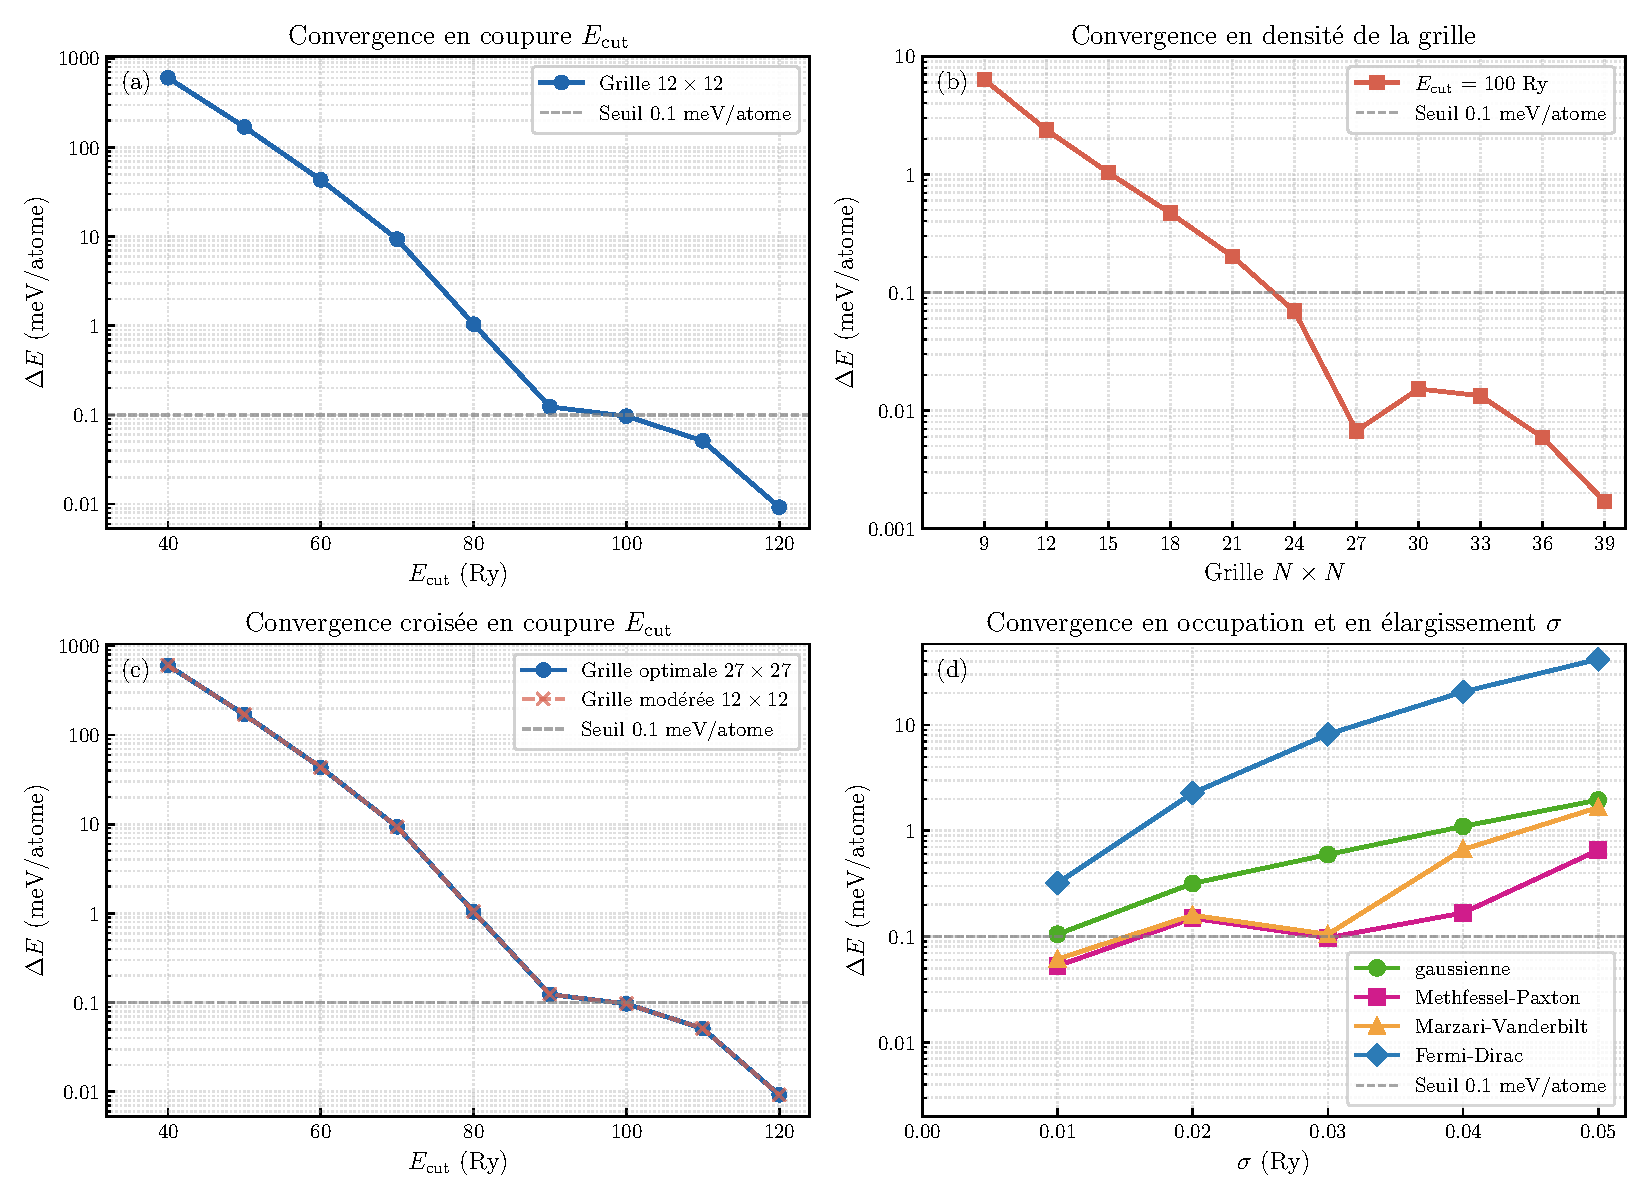
\includegraphics[width=\textwidth]{figures/fig_electron_convergence.pdf}
    \caption[Étude de convergence sur les paramètres physiques affectant l'état fondamental des électrons dans une feuille de graphène parfaite.]{Tests de convergence de l'énergie totale du graphène parfait. (a) Convergence de la coupure $E_\text{cut}$ avec une grille $12\times 12$. (b) Convergence de la grille avec $E_\text{cut}=100$~Ry. (c) Convergence de la coupure $E_\text{cut}$ avec la grille $27\times 27$. (d) Convergence du schéma d'occupation en fonction de l'élargissement $\sigma$ avec $E_\text{cut}=100$~Ry et une grille $27\times 27$. Le seuil de convergence est $0.1$~meV par atome pour tous les tests.}
    \label{fig:convergence_dft}
\end{figure}
\vspace*{\fill}
\clearpage
\section{Paramètres des calculs}\label{sec:annexe_param_dft}
\vspace*{\fill}
\begin{table}[H]
    \centering
    \caption[Paramètres du calcul DFT de la cellule unitaire.]{Paramètres du calcul DFT de la cellule unitaire du graphène parfait (chapitre~\ref{chap:théorie}).}
    \label{tab:param_dft}
    \small
    \setlength{\tabcolsep}{4pt}
    \begin{tabular}{p{0.27\textwidth} p{0.46\textwidth} p{0.14\textwidth}}
        \hline\hline
        Paramètre & Valeur & Section \\
        \hline
        Code & \texttt{QuantumESPRESSO} & \ref{sec:electron_results} \\
        Fonctionnelle d'échange-corrélation & PBE & \ref{sec:electron_results} \\
        Pseudo-potentiel & ONCV \textit{stringent} pour le carbone, bibliothèque PseudoDojo & \ref{sec:electron_results} \\
        Coupure $E_\text{cut}$ & $100$~Ry & \ref{sec:electron_results} \\
        Grille $\kv$ & $27\times 27$, centrée sur $\Gamma$ & \ref{sec:electron_results} \\
        Occupation & Marzari-Vanderbilt, $\sigma = 0.01$~Ry & \ref{sec:electron_results} \\
        Diagonalisation & Davidson & \ref{sec:electron_results} \\
        \textit{Mixing} & Broyden, $\beta = 0.3$ & \ref{sec:electron_results} \\
        Seuil de convergence SCF & $10^{-14}$~Ry & \ref{sec:electron_results} \\
        Critère des tests de convergence & $0.1$~meV par atome & \ref{sec:electron_results} \\
        Paramètre de maille $a$ & $2.466$~\AA{}, par relaxation structurelle & \ref{sec:electron_results} \\
        Cellule de vide & 30 bohr & \ref{sec:electron_results}\\
        Troncature de Coulomb & 2D & \ref{sec:electron_results}\\
        \hline\hline
    \end{tabular}
\end{table}
\vspace*{\fill}
\clearpage
\vspace*{\fill}
\begin{table}[H]
    \centering
    \caption[Paramètres des calculs DFPT et des phonons.]{Paramètres des calculs DFPT et des phonons du graphène parfait (chapitres~\ref{chap:théorie} et~\ref{chap:eph}).}
    \label{tab:param_dfpt}
    \small
    \setlength{\tabcolsep}{4pt}
    \begin{tabular}{p{0.27\textwidth} p{0.46\textwidth} p{0.14\textwidth}}
        \hline\hline
        Paramètre & Valeur & Section \\
        \hline
        Grille $\kv$ du calcul DFT préalable & $24\times 24$, centrée sur $\Gamma$ & \ref{sec:phonon_results} \\
        Grille $\qv$ de la DFPT & $24\times 24$ & \ref{sec:phonon_results} \\
        Occupation & Marzari-Vanderbilt, $\sigma = 0.02$~Ry & \ref{sec:phonon_results} \\
        Coupure $E_\text{cut}$ & $100$~Ry & \ref{sec:g_détails} \\
        Paramètre de maille & $2.466$~\AA & \ref{sec:g_détails} \\
        Cellule de vide & $30$~bohr & \ref{sec:g_détails} \\
        Troncature de Coulomb & bidimensionnelle & \ref{sec:g_détails} \\
        Seuil de convergence (DFT et DFPT) & $10^{-14}$~Ry & \ref{sec:g_détails} \\
        Chemin d'interpolation & $\Gamma\to K\to M\to\Gamma$, $125$ points par segment & \ref{sec:phonon_results} \\
        Densité d'états : grille $\qv$ & $500\times 500$ & \ref{sec:phonon_results} \\
        Densité d'états : élargissement & gaussien, $3$~cm$^{-1}$ & \ref{sec:phonon_results} \\
        \hline\hline
    \end{tabular}
\end{table}
\vspace*{\fill}
\clearpage
